\chapter{DUNE Far Site Technical Coordination}
\label{ch:exec-tc}

%%%%%%%%%%%%%%%%%%%%%%%%%%%%%%%%%%%%%%%%%%%%%
\section{Overview}

Far site \dword{tc} concerns the organization and management of 
activities required to design, construct,
fabricate, install, and commission the \dword{dune} \dword{fd} modules. 
      The \dword{dune} collaboration has direct responsibility for the design 
and construction of the \dword{dune} detectors.  Groups of collaboration 
institutes, referred to as ``consortia,'' assume responsibility for 
the different detector subsystems.  The activities of the consortia are 
overseen and coordinated through the \dword{dune} \dword{tc} organization 
headed by the \dword{dune} \dword{tcoord}.  The \dword{tc} organization 
provides project support functions such as safety coordination, 
engineering integration, change control, document management, scheduling, 
risk management, and technical review planning.  \dword{dune} \dword{tc} 
manages internal, subsystem-to-subsystem interfaces and is responsible 
for ensuring the proper integration of the different subsystems.   

\dword{dune} \dword{tc} works closely with the support teams of its 
\dword{lbnf-dune} partners within the framework of the \dword{jpo} to 
ensure coherency in project support functions across the entire global 
enterprise.  To ensure the consistency of the \dword{dune} \dword{esh} 
and \dword{qa} programs with those across \dword{lbnf-dune}, the 
\dword{lbnf-dune} \dword{esh} and \dword{qa} managers, who sit within 
the \dword{jpo}, are also embedded within the \dword{dune} \dword{tc} 
organization.  The \dword{jpo} establishes the global engineering
and documentation requirements adhered to within the \dword{dune} 
\dword{fd} construction project, manages external \dword{dune} detector 
interfaces with \dword{lbnf}, and is responsible for ensuring proper 
integration of the \dword{dune} detector elements within the facilities 
and supporting infrastructure.  

The \dword{jpo} organization will evolve over time to incorporate the 
on-site team responsible for coordinating integration and installation 
activities at \dword{surf} under the direction of the \dword{ipd}.  
Detector integration and installation activities are supported by the 
\dword{dune} consortia, which maintain responsibility for ensuring 
proper installation and commissioning of their subsystems.  External 
\dword{dune} interfaces with the on-site integration and installation 
activites are managed through the \dword{jpo}.

%%%%%%%%%%%%%%%%%%%%%%%%%%%%%%%%%%%%%%%%%%%%%
\section{Far Site Integration Organization}
\label{sec:exec-tc-partners}

The \dword{lbnf} project is responsible for providing both the 
conventional facilities and supporting infrastructure (cryostats 
and cryogenic systems) that house the \dword{dune} \dword{fd} 
modules.  
The international \dword{dune} 
collaboration under the direction of its management team is 
responsible for the production of the \dword{fd} components.  The 
\dword{dune} \dword{fd} construction project encompasses all 
activities required for designing and fabricating the different 
detector elements and incorporates contributions from a number 
of international partners including the U.S. \dword{doe}.  
The global structure of \dword{lbnf-dune}, which encompasses 
both project elements, is based heavily on 
the organization that successfully executed the construction,
installation, commissioning and operation of the \dword{protodune}
detectors at \dword{cern}. 
The 
%global 
far site integration organization of the \dword{lbnf-dune} is shown in Figure~\ref{fig:fs-integration-org-chart}. 

\begin{dunefigure}[Global project organization]{fig:fs-integration-org-chart}
  {\dword{lbnf-dune} organization.}
  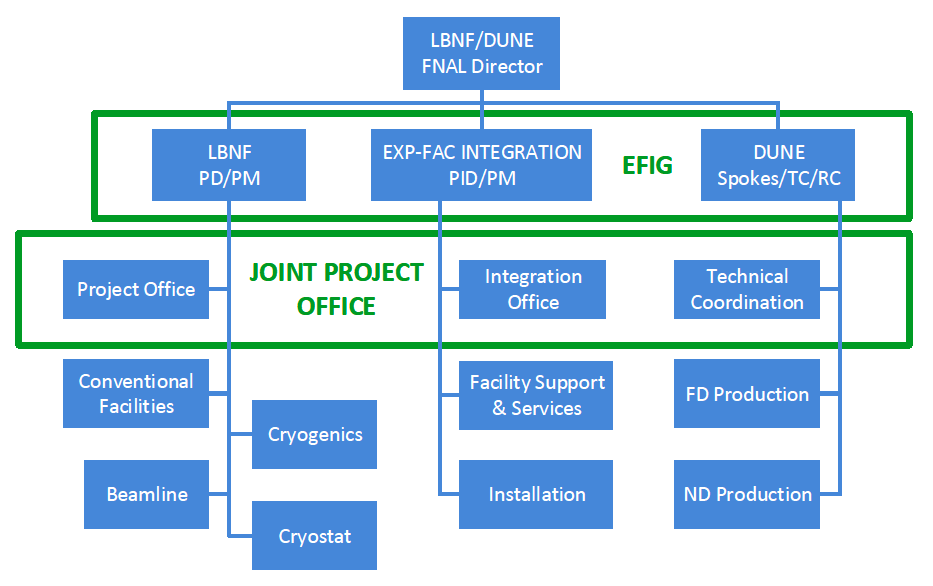
\includegraphics[width=0.99\textwidth]{fs-integration-org-chart} %DUNE_global}
\end{dunefigure}

In addition to the \dword{lbnf} and \dword{dune} pieces, the 
overall coordination of integration and installation activities 
in the excavated, underground caverns is managed as a separate
element of \dword{lbnf-dune} under the responsibility of 
the \dword{ipd}, who is appointed by and reports directly to the 
\dword{fnal} director.  To ensure the best possible coordination 
across all elements of \dword{lbnf-dune}, the \dword{ipd} connects 
to both the facilities and detector construction projects through 
ex-officio positions on the \dword{lbnf} Project Management Board 
and \dword{dune} \dword{exb}, respectively.

The \dword{efig} is the body responsible for the required high-level
coordination between the \dword{lbnf} and \dword{dune} construction 
projects.  The \dword{lbnf} Project Director and \dword{ipd} 
co-chair the \dword{efig}.  This group is responsible for steering the integration and 
installation of the \dword{lbnf-dune} pieces and operates via the 
consensus of its leadership team. 

The \dword{efig} is augmented by a \dword{jpo} that supports the
\dword{lbnf} and \dword{dune} projects as well as the integration
effort across \dword{lbnf} and \dword{dune}. The \dword{jpo} 
combines project activities and functions that exist within the 
\dword{lbnf} and \dword{dune} projects to ensure that they are 
properly coordinated across the entire enterprise.    
To achieve coherency in the review process across the 
\dword{lbnf-dune} enterprise, reviews will be coordinated 
through the \dword{jpo}. 
Figure~\ref{fig:DUNE_jpo} shows the current organizational 
structure of the \dword{jpo}, indicating the members being 
pulled in from the \dword{lbnf} (LBNF), \dword{dune} (TC), and 
\dword{lbnf}/\dword{dune} Integration and Installation (NP) 
project teams.

\begin{dunefigure}[JPO organization chart]{fig:DUNE_jpo}
  {\dword{jpo} organization chart}
  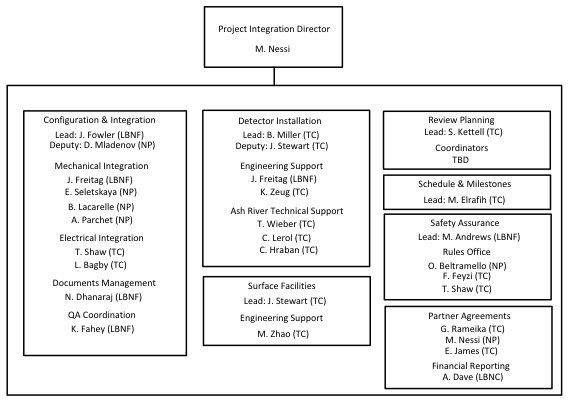
\includegraphics[width=0.99\textwidth]{DUNE_jpo}
\end{dunefigure}


\subsection{Safety}
\label{sec:dune_safety}

To ensure a consistent approach to safety across \dword{lbnf-dune},
a single project \dword{esh} manager reports directly 
to the \dword{lbnf} project director, \dword{ipd}, and \dword{dune}
management (via the \dword{dune} \dword{tcoord}).  This individual
directs separate safety teams responsible for implementing the 
\dword{lbnf-dune} \dword{esh} program within both the \dword{lbnf} 
and \dword{dune} projects as well as the \dword{lbnf}/\dword{dune}
integration and installation activities at \dword{surf}.  The 
project \dword{esh} manager works directly with the \dword{fnal} 
and \dword{surf} safety teams to ensure that all project-related 
activities comply with the rules and regulations of the host 
organizations.  The Project \dword{esh} manager works with a \dword{jpo} 
engineering safety assurance team to develop
equivalencies in codes and standards across the international project
as needed.

Safety issues related to the handling 
and installation of components are addressed starting 
from the earliest design reviews through the development 
of detailed engineering notes containing the required
structural analysis.


\subsection{Engineering Integration}
\label{sec:dune_engineering}

\fixme{it sounds like there are a few different engineering teams, right? Anne}

A central \dword{jpo} engineering team is responsible for building 
an integrated model of the detectors within their supporting
infrastructure and the \dword{cf} that house them.  
The \dword{lbnf-dune} project has adopted 
the formal change control process developed previously for the 
\dword{lbnf} project.  The change control process applies to 
proposed modifications of requirements, technical designs, 
schedule, overall project scope and assigned responsibilities 
for individual scope items. 
The \dword{jpo} team incorporates approved design changes as they 
are received and runs a series of checks to ensure that no errors 
or spatial conflicts are introduced into the model. After receiving the 
appropriate sign-offs from all parties, 
The \dword{jpo} team is responsible for maintaining  
each release  of the model and making it available to the 
design teams as the current release against which the next set 
of design changes is to be generated. 

Electrical engineers are also incorporated within the central
\dword{jpo} team to ensure proper integration and installation 
of the detector electrical components.  

The \fixme{another?} \dword{jpo} engineering team is responsible for documenting and
controlling the interfaces between the \dword{lbnf} and \dword{dune} 
projects as well as the interfaces between these projects and the 
\dword{lbnf}/\dword{dune} integration and installation activities 
at \dword{surf}.  

\fixme{can we add a bit about risks here?}

\subsection{Schedule and Milestones}
\label{sec:dune_schedule}

The \dword{jpo} team is responsible for creating a single 
project schedule for \dword{lbnf-dune} incorporating all 
\dword{lbnf} and \dword{dune} activities together with the 
integration and installation activities at \dword{surf} 
incorporating all interdependencies.  This schedule will 
be used to track the status of the global enterprise.  
  The non-\dword{doe} activities 
will not be tracked using the formal \dword{evms} procedures 
required for the \dword{doe} project activities but rather 
through regular assessments of progress towards completion 
by the management teams responsible for those activities.  


\subsection{Partner Agreements and Financial Reporting}
\label{sec:dune_agreements}

Partner contributions to all project elements will be detailed 
in a series of written agreements.  \dword{dune} will create a single \dword{mou} 
detailing the contributions of all participating partners.  
 The  \dword{jpo} will coordinate a series of more technical agreements, describing the exact 
boundaries between partner contributions and the terms and 
conditions under which they will be delivered will accompany
 the primary agreements.   

%%%%%%%%%%%%%%%%%%%%%%%%%%%%%%%%%%%%%%%%%%%%%
\section{Detector Design and Construction Organization}
\label{sec:es-tc-det-const}

The \dword{dune} \dword{fd} construction project refers collectively 
to the activites associated with the design and construction of the
necessary detector components.  \dword{dune} collaboration management 
is responsible for overseeing this portion of \dword{lbnf-dune} and 
ensuring its successful execution.  The high-level \dword{dune} 
collaboration management team consisting of the co-spokespersons, 
\dword{tcoord}, and \dword{rcoord} is responsible for the day-to-day 
administration of the project.  

Construction of the \dword{dune} \dwords{fd} is carried out by 
consortia of collaboration institutions who assume responsibility 
for detector subsystems. Each consortium plans and executes the 
construction, installation and commissioning of its subsystem.  In most cases a single consortium is responsible for subsystem deliverables that are supported by 
multiple funding agencies, with each agency managing its own internal projects. 

Each consortium has an overall consortium leader 
and a technical lead.  The consortium leader chairs an institutional 
board composed of one representative from each of the collaborating 
institutions contributing to the activities of the consortium.  Major 
consortium decisions such as technology selections and assignment of 
responsibilities within the institutions are passed through its institutional 
board.  These decisions are then passed as recommendations to 
the \dword{dune} \dword{exb} for formal collaboration approval.

Because the consortia operate as self-managed entities, a strong
\dword{tc} organization is required to ensure overall integration 
of the detector elements and successful execution of the detector
construction project.  \dword{tc} areas of responsibility include 
general project oversight, systems engineering, \dword{qa}, and 
safety.  \dword{tc} also supports the planning and execution 
of integration and installation activities at \dword{surf} (see 
Chapter~\ref{ch:tc-jpo}).  

The \dword{tcoord} manages the overall detector construction project
through regular board meetings with the consortium leadership teams 
and members of the \dword{tc} organization (see Section~\ref{sec:tc}).  
These board meetings are used to identify and resolve technical issues
and serve as the primary forums for required interactions between the 
consortia. Any decisions generated through these board meetings are passed to 
the \dword{dune} \dword{exb} as recommendations for formal approval.

The \dword{tcoord} heads an organization that supports the work of 
the consortia and has responsibility for a number of major project 
support functions including:
\begin{itemize}
\item ensuring that each consortium has a well defined and complete
  scope, that interactions between consortia are sufficiently 
  well defined, and that any required scope sitting outside of the 
  consortia is provided through other sources such as collaboration
  common funds;
\item defining and documenting scope boundaries and technical 
  interfaces both between consortia and with \dword{lbnf};  
\item developing an overall schedule with appropriate dependencies
  between activities covering all phases of the project. 
\item ensuring that appropriate engineering and safety standards 
  are developed, understood, and agreed to by all key stakeholders 
  and that these standards are conveyed to and understood by each
  consortium;
\item ensuring that all \dword{dune} requirements on \dword{lbnf} 
  for \dword{cf}, cryostat and cryogenics are clearly defined and 
  agreed to by each consortium;
\item ensuring that each consortium has well developed and reviewed
  component designs, construction plans, \dword{qc} processes, and 
  safety programs; and
\item monitoring the overall project schedule and the progress of 
  each consortium towards delivering its assigned scope. 
\end{itemize}

The \dword{dune} \dword{tc} organizational structure is shown 
in Figure~\ref{fig:DUNE_tc}.  

\begin{dunefigure}[DUNE Technical Coordination org chart]{fig:DUNE_tc}
  {\dword{dune} \dword{tc} Organizational Chart}
  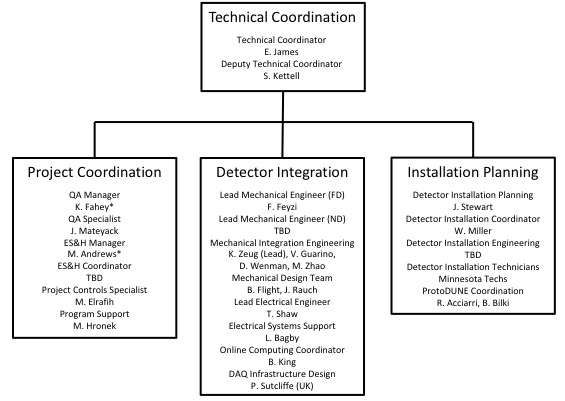
\includegraphics[width=0.99\textwidth]{DUNE_tc}
\end{dunefigure}
\fixme{figure \ref{fig:DUNE_tc} a bit fuzzy}

The \dword{tc} project coordination team incorporates \dword{esh}, 
\dword{qa}, and project controls specialists.  Engineering support 
is provided through the \dword{tc} detector integration team 
headed by the lead \dword{dune} mechanical and electrical engineers.
Planning coordinators for integration and installation activities 
at \dword{surf} are embedded within both the \dword{jpo} and the 
\dword{tc} installation planning team.  The dual placement of 
these individuals within both organizations facilitates required 
coordination of the integration and installation planning 
efforts between the core team directing these activities and the 
\dword{dune} consortia, which maintain primary responsibility for 
the individual detector subsystems.  Members of the \dword{tc} 
organization meet weekly to review project progress and discuss 
technical issues. 

The \dword{dune} project has already completed an initial round of design 
and prototyping activities culminating in the construction and operation 
of the \dword{protodune} detectors.  Moving forward, the project is 
updating detector component designs to account for lessons learned from 
the \dword{protodune} experience.  Upon finalization of the designs, the 
project will construct first production versions of all components that 
will be installed and operated in a second phase of \dword{protodune} 
operations prior to the start of full-scale production.  The operation 
of the \dword{protodune2} detectors will follow roughly two years after
the end of operations for the corresponding \dword{protodune} detectors.
In a few cases, the production of long lead-time components will need to 
be started in parallel with the operation of first production components 
in \dword{protodune2}.

%%%%%%%%%%%%%%%%%%%%%%%%%%%%%%%%%%%%%%%%%%%%%
\section{Integration Engineering}
\label{sec:es-coord-integ-sysengr}

Integration engineering for \dword{dune} focuses on three main functions. The first is  configuring the
mechanical and electrical systems of each \dword{detmodule} and managing
the interfaces within them.  The second 
is assuring that the \dwords{detmodule} can be integrated and
installed into their final configuration, and the third is
integrating necessary services provided by \dword{cf} 
with the \dwords{detmodule}. 

To coordinate these functions, the consortia provide engineering data for their
subsystems to the \dword{tc} engineering team, which maintains subsystem
component documentation.  Three-dimensional (\threed) mechanical modeling techniques are well suited 
for representing the \dwords{detmodule} and managing their configurations.
But since  \threed modelling techniques vary, a set
of clear and unambiguous \twod integration drawings must be generated to form
the basis for the \threed model accuracy, as well as the basis for the engineering
design of all components. The \twod integration drawings must show the 
interfaces to the level of detail necessary to ensure proper fit and function.  These \threed and 
\twod are referred to as static because they do not represent effects of gravity, tolerances, cold
temperature, and installation and assembly clearances.

For installation and operation, however, ``envelope'' models  are developed to 
address effects on the detector 
caused by e.g., distortion of the cryostat and \dword{dss} due to gravity, loads  during 
detector filling and operation, thermal contraction,  and effects of tolerances, clearances for tooling, and so on.

Many interfaces among components must be controlled by \dword{tc}. Interfaces are developed, managed, and controlled through additional models and drawings. 
Integration drawings are derived directly from the overall
integration model, which in turn is assembled from
component models developed by the consortia.

TO BE CONTINUED
